\documentclass[nonacm,sigconf,natbib=false]{acmart}

%%
%% \BibTeX command to typeset BibTeX logo in the docs
\AtBeginDocument{%
  \providecommand\BibTeX{{%
    Bib\TeX}}}

%%
%% The majority of ACM publications use numbered citations and
%% references, obtained by selecting the acmnumeric BibLaTeX style.
%% The acmauthoryear BibLaTeX style switches to the "author year" style.
%%
%% If you are preparing content for an event
%% sponsored by ACM SIGGRAPH, you must use the acmauthoryear style of
%% citations and references.
%%
%% Bibliography style
\RequirePackage[
  datamodel=acmdatamodel,
  style=acmnumeric,
  ]{biblatex}

%% Remove auto generated acm text
\setcopyright{none}
\settopmatter{printacmref=false} % Removes citation information below abstract
\renewcommand\footnotetextcopyrightpermission[1]{} % removes footnote with conference information in first column
\pagestyle{plain}

%% Declare bibliography sources (one \addbibresource command per source)
\addbibresource{linear_agreement_and_liveness.bib}

%%
%% end of the preamble, start of the body of the document source.
\begin{document}

%%
%% The "title" command has an optional parameter,
%% allowing the author to define a "short title" to be used in page headers.
\title{Auswirkungen von Optimierungen in Konsensprotokollen auf die Systemstabilität} % Original: Linear Agreement and Liveness 

%%
%% The "author" command and its associated commands are used to define
%% the authors and their affiliations.
\author{Eugen Becker}
\email{eugen.becker@fau.de}
\affiliation{%
  \institution{Friedrich-Alexander-Universität Erlangen-Nürnberg}
  \streetaddress{}
  \city{}
  \state{}
  \postcode{}
  \country{}
}

%%
%% By default, the full list of authors will be used in the page
%% headers. Often, this list is too long, and will overlap
%% other information printed in the page headers. This command allows
%% the author to define a more concise list
%% of authors' names for this purpose.
\renewcommand{\shortauthors}{Eugen Becker}

%% Change abstract heading to Kurzfassung
\renewcommand{\abstractname}{Kurzfassung}

%% Change the bibliography title
\renewcommand{\refname}{Bibliographie}

%%
%% The abstract is a short summary of the work to be presented in the
%% article.
\begin{abstract}
  To do ...

  To do ...

  To do ...

  To do ...

  To do ...

  To do ...

  To do ...

  To do ...

  To do ...

  To do ...

  To do ...

  To do ...
\end{abstract}

%%
%% Keywords. The author(s) should pick words that accurately describe
%% the work being presented. Separate the keywords with commas.
%%\keywords{Do, Not, Us, This, Code, Put, the, Correct, Terms, for,
%%  Your, Paper}

%%
%% This command processes the author and affiliation and title
%% information and builds the first part of the formatted document.
\maketitle

\section{Einleitung}
To do ...

To do ...

To do ...

To do ...

To do ...

To do ...

To do ...

To do ...

To do ...

To do ...

To do ...

To do ...

To do ...

To do ...

To do ...

To do ...

To do ...

To do ...

To do ...

To do ...

To do ...

To do ...

To do ...

To do ...

To do ...

To do ...

To do ...

To do ...

To do ...

To do ...

To do ...

To do ...

To do ...

To do ...

To do ...

To do ...

To do ...

To do ...

To do ...

To do ...
\section{Grundlagen}
In diesem Kapitel wird Grundwissen vermittelt, das für das Verständnis dieser Arbeit benötigt wird. Dabei werden zunächst die Begriffe State Machine Replication und Byzantinische Fehler näher betrachtet und zum Schluss das vorausgesetzte System Modell beschrieben.

\subsection{State Machine Replication}

Ein bewährter Ansatz, um zuverlässige Dienste zu implementieren, ist State Machine Replication (SMR)\cite{smr-lamport}\cite{smr-schneider}. Bei diesem Ansatz wird Fehlertoleranz dadurch erreicht, dass ein Dienst als Zustandsmaschine auf mehrere Server repliziert wird, die zusammen ein verteiltes System bilden. Dieses System verhält sich für Clients wie ein einzelner zentraler Dienst, der alle Clientbefehle nacheinander ausführt. Wird der SMR-Ansatz korrekt implementiert, garantiert er die folgenden zwei Eigenschaften:
\begin{itemize}
  \item \textbf{Safety (Sicherheit)}: Alle korrekten Replikate führen dieselbe Abfolge von Operationen auf ihrer Zustandsmaschine aus.
  \item \textbf{Liveness (Lebendigkeit)}: Alle angeforderten Clientbefehle werden innerhalb einer angemessen Zeit ausgeführt.
\end{itemize}

Bei der Liveness Property nochmal schauen, weil eigentlich heißt es ja, dass das System fortschreitet und nicht ins Stocken kommt. Eventuell überarbeiten.

Die Implementierung des SMR-Ansatzes gemäß \cite{smr-schneider} setzt deterministische Zustandsmaschinen voraus. Das heißt alle korrekten Replikate starten im selben Zustand und gehen bei gleichen Clientbefehlen in den gleichen Zustand über. Um die Sicherheit im SMR-System zu gewährleisten, müssen sich alle korrekten Replikate auf eine einheitliche Reihenfolge einigen, in der sie die Clientoperation auf ihrer Zustandsmaschine ausführen. Hierzu wird ein Konsensalgorithmus verwendet, der sicherstellt, dass trotz fehlerhafter Replikate eine Einigung erzielt und dem Client geantwortet wird.

Es existieren eine Vielzahl unterschiedlicher SMR-Protokolle, die sich in ihrem Konsensalgorithmus und der Art und Weise, wie sie die Lebendigkeit des Systems sicherstellen, unterscheiden. In dieser Arbeit werden die beiden Protokolle Practical Byzantine Fault Tolerance (PBFT)\cite{pbft} und HotStuff\cite{hotstuff} näher betrachtet.

Hier noch Quorumzertifikat erklären...
Eventuell sagen, dass ein Konsensalgorithmus aus mehreren Phasen besteht, in der ersten wird ein Vorschlag gemacht, dann voten alle und dann führen alle das Ergebnis aus (commit).

\subsection{Byzantinische Fehlertoleranz}

In einem verteilten System können verschieden Arten von Fehlern auftreten. Typisch sind dabei zum Beispiel Serverausfälle oder Kommunikationsfehler, die durch Netzwerkprobleme verursacht werden. Bei Fail-Stop Fehlern\cite{smr-schneider} geht ein Replikat, bevor es aufgrund eines Fehlers stoppt, in einen Zustand über, der anderen Replikaten signalisiert, dass ein Fehler aufgetreten ist. Ein Server kann aber auch bei einem Crash Fehler in einem willkürlichen Zustand stoppen. Bei Kommunikationsfehlern können Nachrichten aufgrund von Netzwerkproblemen verloren gehen, verzögert werden oder in falscher Reihenfolge eintreffen. Allgemein gilt ein Replikat im Kontext von State Machine Replication (SMR) als fehlerhaft, wenn es sich nicht gemäß den Spezifikationen im SMR-Protokoll verhält \cite{smr-schneider}.

Eventuell diese Fail-Stop Geschichte weglassen, interessiert eigentlich niemanden.

Eine besondere Herausforderung stellen Byzantinische Fehler dar, bei denen sich ein Replikat willkürlich oder bösartig gegenüber anderen Replikaten oder dem Client verhalten kann \cite{smr-schneider}. Sie sind schwer zu ermitteln, weil byzantinisch fehlerhafte Replikate nicht immer als fehlerhaft wahrgenommen werden. Beispiele hierfür sind: (1) Absichtliches Versenden falscher oder widersprüchlicher Informationen; (2) Absichtliches Verzögern oder Auslassen von Nachrichten; (3) Gezielte Irreführung ausgewählter Komponenten und korrektes Verhalten gegenüber den restlichen Komponenten; praktisch jedes willkürliche Verhalten ist möglich. Byzantinische Fehler können durch verschiedene Faktoren verursacht werden, wie zum Beispiel Softwarefehler, Hardwareausfälle, Netzwerkprobleme oder böswillige Angriffe.

\subsection{System Modell}

\section{Practical Byzantine Fault Tolerance}

Practical Byzantine Fault Tolerance (PBFT) \cite{pbft} von Castro und Liskov war das erste BFT-SMR-Protokoll, dass in einem partiell synchronen Netzwerk effizient genug war, um in der Praxis eingesetzt zu werden. Im Folgenden wird der Konsensalgorithmus von PBFT vorgestellt und eine Optimierung des Protokolls erläutert. Es wird gezeigt, dass diese Optimierung die Systemlebendigkeit unter einem spezifischen Angriff beeinträchtigt. Abschließend wird eine Lösung präsentiert, um dieses Problem zu beheben.

\subsection{PBFT-Konsensalgorithmus}

Der Konsensalgorithmus von PBFT besteht aus den Phasen \emph{Pre-prepare}, \emph{Prepare} und \emph{Commit} (siehe Abbildung \ref{fig:pbft-normal}). Er beginnt damit, dass ein Client seine Anfrage an alle Replikate im verteilten System sendet.

\textbf{Pre-Prepare-Phase.} Sobald das Anführer-Replikat die Nachricht des Clients erhalten und auf Gültigkeit überprüft hat vergibt es der Nachricht eine Sequenznummer. Diese bestimmt die Reihenfolge, in der Clientoperationen auf allen Zustandsmaschinen ausgeführt werden sollen. Anschließend erstellt es eine Pre-Prepare-Nachricht bestehend aus der Clientoperation, der Sequenznummer und der aktuellen View. Diese Nachricht wird signiert und an alle Backups im System verteilt.

\textbf{Prepare-Phase.} Alle Backups stimmen darüber ab, ob die vom Anführer vorgeschlagene Clientoperation ausgeführt werden soll. Hierzu überprüft jedes Backup die Pre-Prepare-Nachricht auf ihre Gültigkeit und auf mögliche Konflikte mit ihrem aktuellen Zustand und der ursprünglichen Anfrage des Clients. Hat ein Backup die Pre-Prepare-Nachricht akzeptiert, gibt es ihre Stimme ab, indem es eine Prepare-Nachricht an alle anderen Replikate (einschließlich des Anführers) sendet. Jedes Replikat sammelt 2f gültige Prepare-Nachrichten von unterschiedlichen Replikaten (einschließlich seiner eigenen, falls vorhanden). Zusammen mit der Pre-Prepare-Nachricht des Anführers ergibt das ein Quorum von $2f+1$ Stimmen.

\textbf{Commit-Phase.} Hat ein Replikat ein Prepare-Quorum erreicht, signalisiert es dies, indem es eine Commit-Nachricht an alle anderen Replikate sendet. Jedes Replikat sammelt ein Quorum von $2f+1$ gültigen Commit-Nachrichten von unterschiedlichen Replikaten (einschließlich seiner eigenen, falls vorhanden). Hat ein Replikat ein Commit-Quorum erreicht führt es die Operation auf seiner Zustandsmaschine aus und sendet das Ergebnis zurück an den Client.

Ein Client wartet auf $f+1$ übereinstimmende Antworten von unterschiedlichen Replikaten, bevor er die Antwort akzeptiert.

\begin{figure}[htbp]
  \centering
  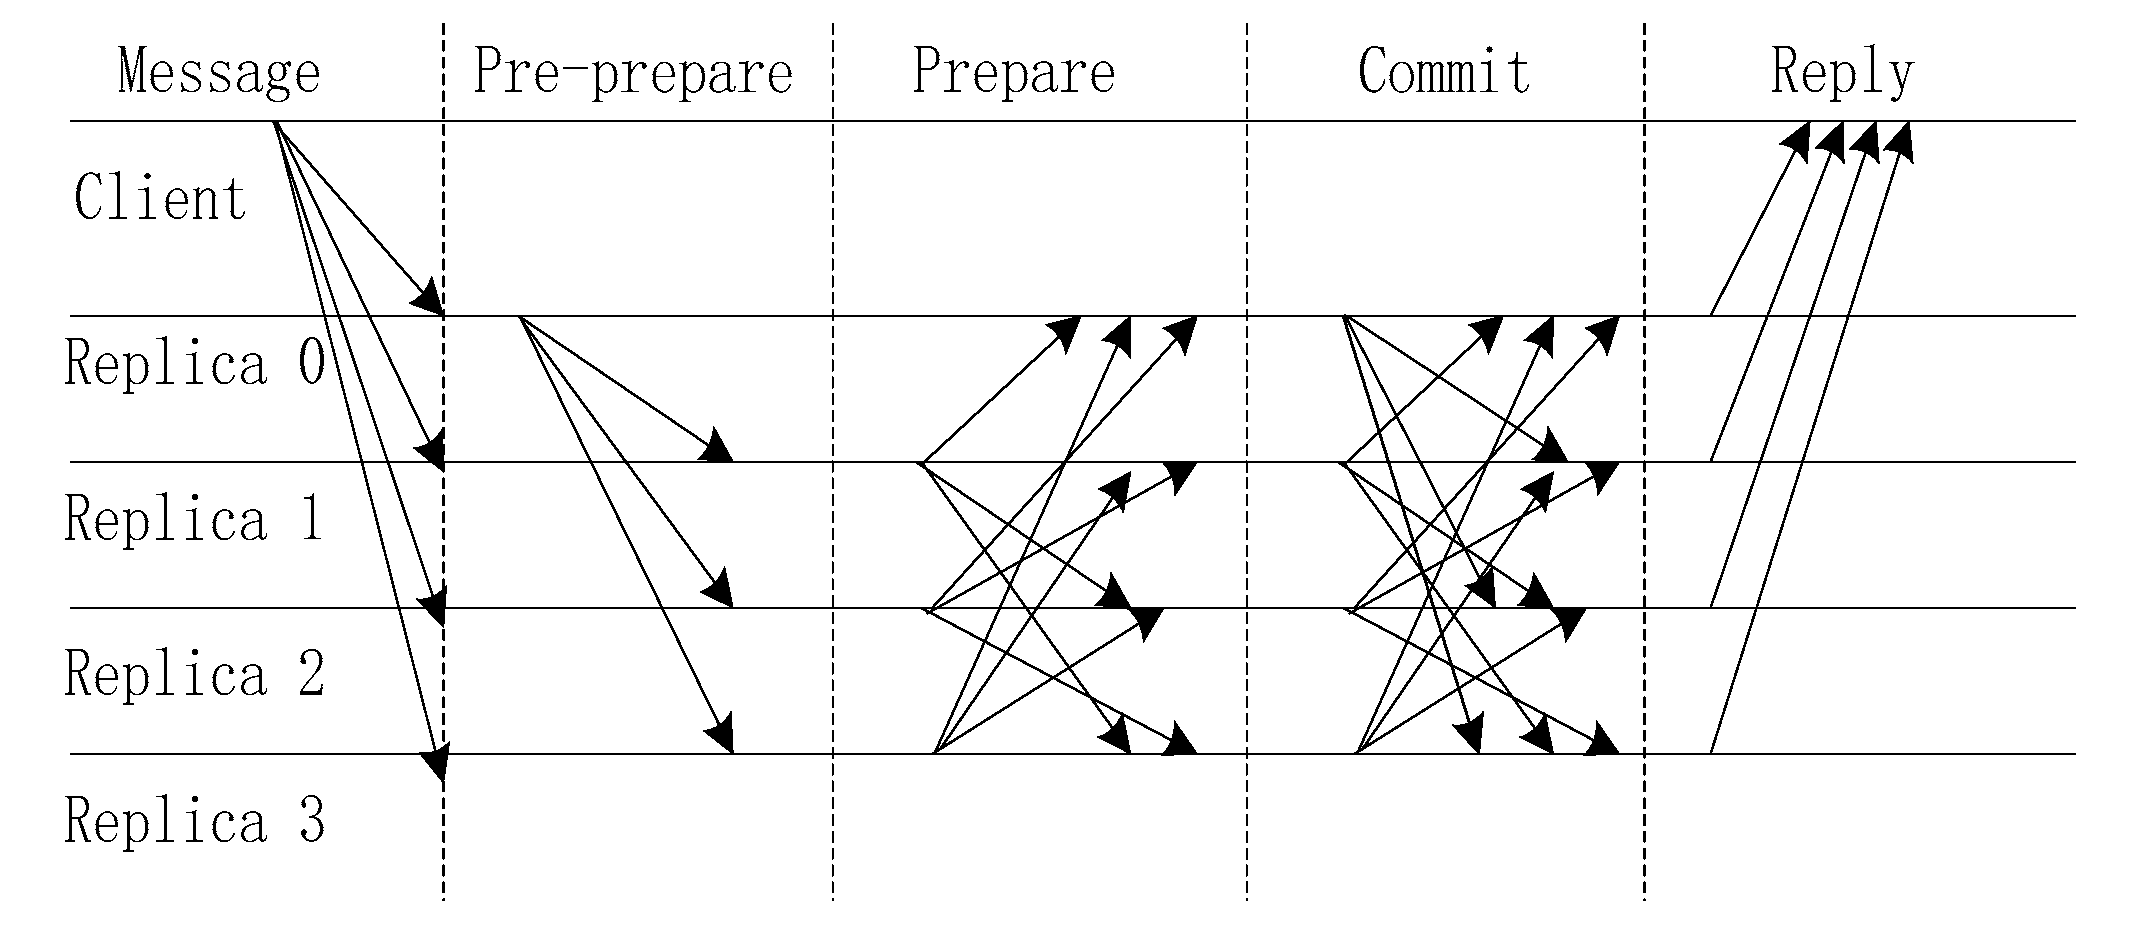
\includegraphics[width=\linewidth]{pbft-normal.png}
  \caption{PBFT-Konsensalgorithmus im fehlerfreien Fall}
  \Description{PBFT-Konsensalgorithmus im fehlerfreien Fall}
  \label{fig:pbft-normal}
\end{figure}

\subsection{Read-Only Optimierung}

Der Konsensalgorithmus von PBFT hat eine hohe Nachrichtenkomplexität von $O(n^2)$. Deshalb haben die Autoren von PBFT mehrere Optimierungen vorgestellt, die das Protokoll effizienter machen sollen \cite{pbft-optimization}. Eine davon ist die Read-Only Optimierung. Sie erlaubt es Leseanfragen ohne Durchlauf des Konsensalgorithmus beantworten zu dürfen. Die Überlegung hierbei ist, dass Leseoperationen den Zustand des Systems nicht verändern und deshalb sofort ausgeführt werden können. Die Read-Only Optimierung setzt allerdings zwei Bedingungen voraus:
\begin{enumerate}
  \item Ein Replikat muss alle vorherigen Operationen festgeschrieben (committed) haben, bevor es eine Read-Only-Anfrage ausführen darf.
  \item Der Client muss bei allen Anfragen auf $2f+1$ übereinstimmende Antworten von unterschiedlichen Replikaten warten, bevor er das Ergebnis akzeptiert, unabhängig davon, ob der Konsensalgorithmus durchlaufen wurde oder nicht. 
\end{enumerate}
Abbildung \ref{fig:pbft-optimization} zeigt, dass ein Client, der wie im normalen Fall nur $f+1$ Antworten akzeptiert, Gefahr läuft, einen veralteten Stand zu lesen. Das liegt daran, dass korrekte Replikate mit der Ausführung festgeschriebener Clientoperationen zurückliegen können und mit einem alten Ergebnis antworten (siehe Abbildung 2a). Zusätzlich kann eine Kombination aus byzantinisch fehlerhaften Replikaten, die absichtlich ein altes Ergebnis liefern, und zurückliegenden korrekten Replikaten dazu führen, dass ein Client trotz $2f+1$ identischer Antworten einen veralteten Stand sieht (siehe Abbildung 2b). Deshalb ist Bedingung (2) auch bei Schreibanfragen notwendig, obwohl diese den Konsensalgorithmus durchlaufen. Wenn ein Client nicht genügend übereinstimmende Antworten erhalten hat, wiederholt er die Leseanfrage als Read-Write-Anfrage, die den Konsensalgorithmus durchlaufen muss.

\begin{figure}[htbp]
  \centering
  \includegraphics[width=\linewidth]{pbft_read_quorum_erklärung.png}
  \caption{Grund}
  \Description{Grund}
  \label{fig:pbft-optimization}
\end{figure}

\subsection{Verlust der Systemlebendigkeit durch Read-Only Optimierung}

Die Bedingung, dass ein Client bei allen Anfragen auf $2f+1$ übereinstimmende Antworten von unterschiedlichen Replikaten warten muss, bevor er das Ergebnis akzeptieren darf, kann bei einem bestimmten Angriff dazu führen, dass die Lebendigkeit des Systems verletzt wird \cite{pbft-liveness-problem}. Der Angriff (siehe Abbildung \ref{fig:read-only-problem}) beinhaltet f byzantinisch fehlerhafte Replikate, darunter den Anfüher und zielt darauf ab, dass kein Client genügend übereinstimmende Antworten sammeln kann. Sobald eine Schreiboperation angefragt wurde, isoliert der Anführer f korrekte Backups, indem er ihnen keine Pre-Prepare Nachricht sendet. 
 
\begin{figure}[htbp]
  \centering
  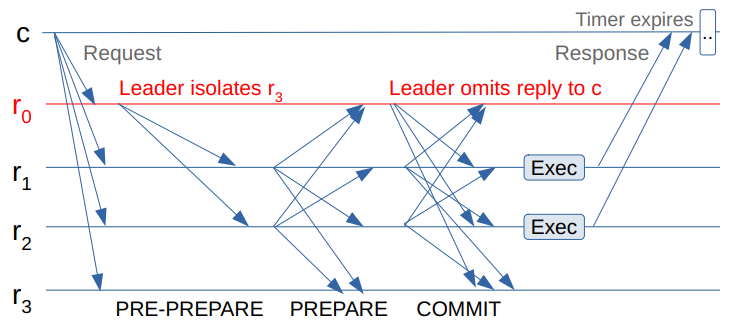
\includegraphics[width=\linewidth]{read-only-problem.png}
  \caption{Grund}
  \Description{Grund}
  \label{fig:read-only-problem}
\end{figure}

\section{HotStuff}

HotStuff\cite{hotstuff} wurde entwickelt, um ein einfaches BFT-SMR-Protokoll bereitzustellen, das hohe Skalierbarkeit bietet. Im Gegensatz zu PBFT, wo jedes Replikat ein Quorum aus signierten Nachrichten unterschiedlicher Replikate sammeln muss, übernimmt bei HotStuff nur der Anführer diese Aufgabe. Aus den Nachrichten der Replikate erstellt der Anführer ein Quorum-Zertifikat (QZ). Ein QZ ist ein Nachweis dafür, dass während einer bestimmten Phase des Konsensalgorithmus ein Quorum von 2f+1 Replikaten für eine Clientoperation gestimmt haben. In HotStuff werden ausstehende Clientbefehle in Blöcken gespeichert. Jeder Block enthält einen oder mehrere Clientbefehle sowie eine Referenz auf seinen Vorgängerblock. Dadurch entsteht eine geordnete Kette von Clientoperationen, die auf allen Zustandsmaschinen ausgeführt werden. Jedes QZ enthält einen zugehörigen Block mit einem oder mehreren Clientoperationen.

\subsection{HotStuff-Konsensalgorithmus}

Der Konsensalgorithmus von HotStuff besteht aus den Phasen \emph{prepare}, \emph{pre-commit}, \emph{commit} und \emph{decide} (siehe Abbildung \ref{fig:hotstuff}). Zu Beginn jeder Prepare-Phase findet ein View-Wechsel statt, wodurch jeder Durchlauf mit einem neuen Anführer startet.

\textbf{Prepare-Phase.} Das neue Anführer-Replikat bekommt von allen anderen Replikaten New-View-Nachrichten geschickt, aus denen es das höchste bekannte Prepare-QZ im System ermittelt. Dieses wird als High-QZ bezeichnet und enthält den aktuellsten Block der Kette an Clientoperationen. Sobald der Anführer eine neue Clientanfrage erhält, erstellt er einen neuen Block mit dieser Anfrage und setzt den Block aus High-QZ als Vorgänger. Anschließend verschickt er eine Prepare-Nachricht an alle Replikate, bestehend aus der aktuellen View, den neuen Block als Vorschlag und High-QZ als Quorum-Nachweis. Jedes Replikat überprüft die Nachricht auf ihre Gültigkeit und akzeptiert den neuen Block, wenn er eine logische Erweiterung der Kette an Clientoperationen darstellt. Hat ein Replikat die Prepare-Nachricht akzeptiert, gibt es ihre Stimme ab, indem es eine Prepare-Vote-Nachricht an den Anführer zurücksendet.

\textbf{Pre-Commit-Phase.} Der Anführer sammelt ein Quorum von 2f+1 Prepare-Vote-Nachrichten und kombiniert diese zu einem Prepare-QZ. Anschließend verschickt er eine Pre-Commit-Nachricht mit dem Prepare-QZ an alle Replikate. Diese antworten mit einer Pre-Commit-Vote-Nachricht.

\textbf{Commit-Phase.} Die Commit-Phase ist ähnlich zur Pre-Commit-Phase. Wenn der Anführer 2f+1 Pre-Commit-Vote-Nachrichten erhalten hat, kombiniert er diese zu einem Pre-Commit-QZ und verschickt es in einer Commit-Nachricht an alle Replikate. Diese antworten mit einer Commit-Vote-Nachricht. In dieser Phase sperrt ein Replikat seinen Zustand auf dem vorgeschlagenen Block. Das heißt es akzeptiert nur noch einen neuen Block, wenn er den aktuell gesperrten Block als Vorgänger hat oder sich in einer höheren View befindet als dieser. Das ist notwendig, damit keine widersprüchlichen Clientoperationen akzeptiert werden können (Sicherheitsgarantie).

\textbf{Decide-Phase.} Sobald der Anführer ein Quorum aus Commit-Vote-Nachrichten gesammelt hat, kombiniert er diese zu einem Commit-QZ und verschickt es in einer Decide-Nachricht an alle Replikate. Durch die Decide-Nachricht weiß ein Replikat, dass der vorgeschlagene Knoten bzw. Clientbefehl festgeschrieben (committed) und auf der Zustandsmaschine ausgeführt werden darf. Nachdem es die Antwort an den Client gesendet hat, erhöht es den View-Zähler und startet eine neue View durch das Versenden einer New-View-Nachricht an den neuen Anführer.

Ebenso wie in PBFT wartet der Client auf f+1 identische Antworten von unterschiedlichen Replikaten, bis er eine Antwort akzeptiert.

\begin{figure}[htbp]
  \centering
  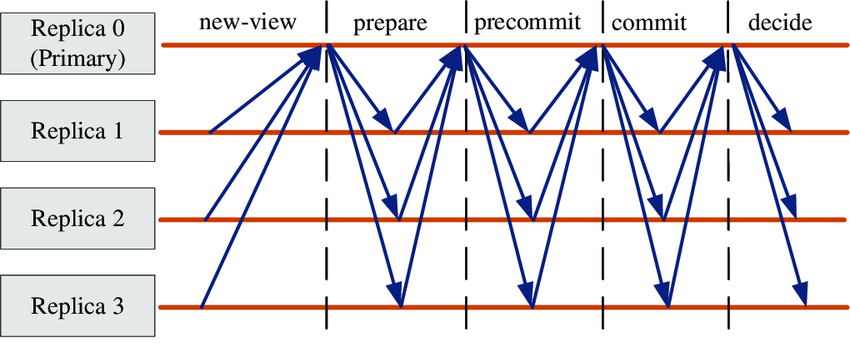
\includegraphics[width=\linewidth]{hotstuff.png}
  \caption{Grund}
  \Description{Grund}
  \label{fig:hotstuff}
\end{figure}

\subsection{Chained HotStuff}

Betrachtet man die einzelnen Phasen des HotStuff Konsensalgorithmus, dann fällt auf, dass sie sich sehr ähneln. In jeder Phase werden sammelt der Anführer genügend Vote-Nachrichten, um ein Quorumzertifikat zu bilden. Die Autoren von HotStuff machen sich diese 


%%
%% Print the bibliography
%%
\printbibliography

\end{document}
\endinput
